\chapter{电池 OBD 系统设计}
\label{chap:OBD}

\section{OBD 系统简介}
在当前社会,车辆作为人们日常使用最多,普及程度最高的交通运输工具之一,已经发展成为一个拥有机械和电子技术复杂的体系,而对于汽车上存在的诸多部件,在过去,各个汽车生产商采用不同的诊断方法,而采用传统的诊断方法无法做到对于故障的及时诊断与回报,用户无法直接了解汽车是否故障,也无法判断车子的故障状态,只有将车辆送回维修厂,使用专业的诊断仪器才能够了解故障状态;在政府方面,汽车采用不同的诊断系统也无法形成一个系统化的监管制度,如何做到汽车的故障统一,系统的故障诊断的过程标准化,故障项目标准化,在这种情况下车载诊断系统,又被称作 OBD(On Board Diagnosis)系统,首先被美国提出的标准化诊断系统,被推广至今,已经成为一个统一的诊断系统,该系统会在指定的时间间隔内监控车辆的运行状态,并且通过对于来自传感器的数据进行储存,分析,诊断出是否存在故障。一旦车辆的某一个子系统或者部件产生了问题,OBD 系统就会通过内部的数据库检查故障的类型和严重程度,在某一条件符合的情况下,将会产生故障代码,储存在系统的非易失性储存其中,并且通过汽车总线发送提醒讯号(MIL 灯)通知驾驶员和汽车维修厂的维修人员。

OBD-II 与第一代的 OBD 系统相比,统一了 OBD 系统的物理接口,以及引脚,并且在物理接口处提供了给外部诊断仪器的供电的引脚,当外部的诊断仪插入后,不需要额外的供电,就可以运行,简化了诊断的过程。同时 OBD 协议也规定了一个标准的电气信号传输格式,以及传输的内容,在原有的仅能够支持故障的诊断相比,增加了实时监控车辆的运行数据的功能,虽然 OBD-II 标准的目标是提供车辆排放方面的诊断,但是目前的大多数汽车制造厂商会将 OBD 系统放置在整车网络上,使得所有的设备都能够被同时诊断故障。

一个基本的车载 OBD 系统如图 \ref{fig:OBD_structure} 所示。汽车的 MIL 灯(Malfunction Indicator Lamp)通常情况下由汽车的 VCU(整车电子控制单元)控制,在平常的适用情况下,OBD 系统将会采集来自于传感器的数据并将数据分类暂时储存,以便使用,并在同时对数据进行诊断,对于故障进行分类储存。而当系统发生故障之后,对应子系统的 OBD 系统将会上报故障给 VCU,VCU 通过已经上报的故障进行判断是否进行 MIL 灯的点亮。而在故障发生后,检测人员将会使用诊断仪读取已经储存的数据,包括故障发生时的传感器数据,时间,和故障的相关信息,在维修后通过诊断仪也可以发送指令给对应的 OBD 系统,进行储存故障信息的清除,熄灭车辆的 MIL 故障灯。

\begin{figure}
	\centering
	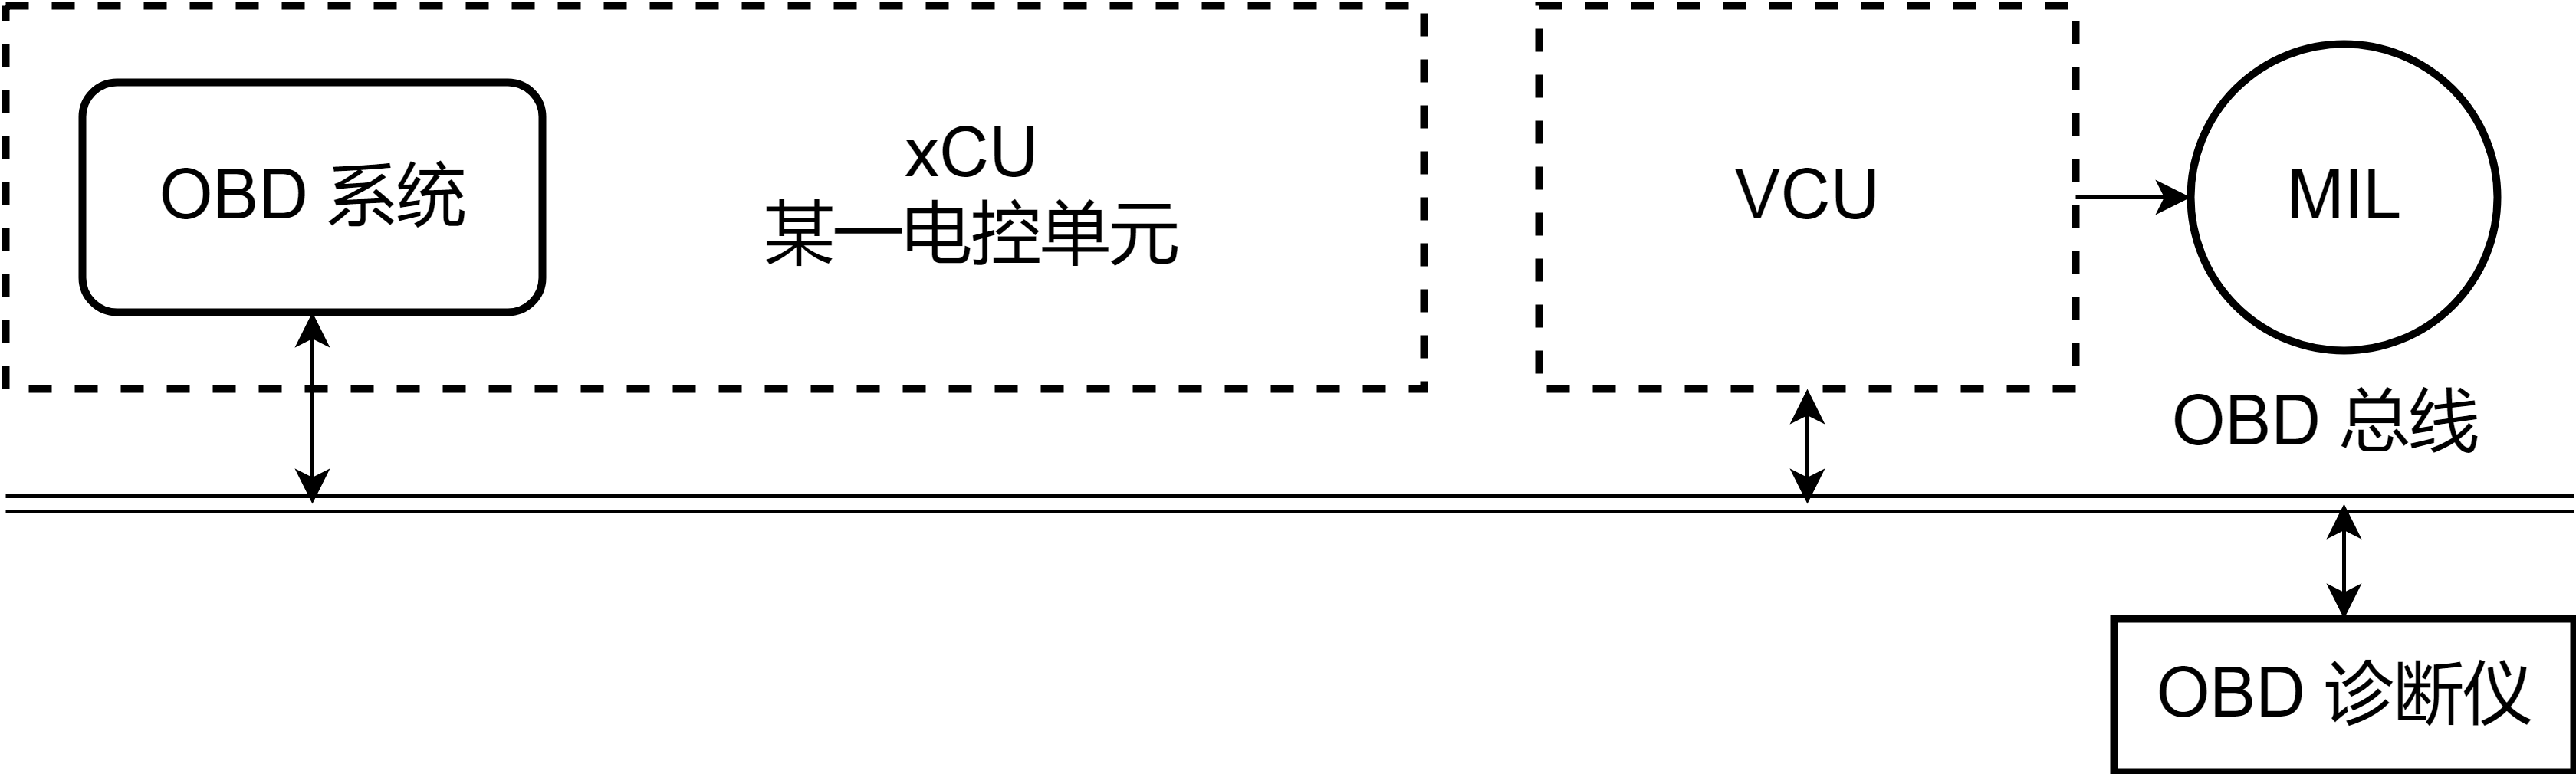
\includegraphics[width=0.7\textwidth]{figures/OBD_structure.png}
	\caption{新能源汽车的 OBD 系统结构}\label{fig:OBD_structure}
\end{figure}

随着目前的计算机技术发展,目前的车载诊断系统已经具备多种多样的功能,譬如在汽车总线之外,还能够通过多种信息传输介质来进行信息的传输,这时由于 OBD 系统仅仅规定了标准化的信息传输协议,而没有限定信息传输的介质,在未来,OBD 系统将会基于更加高速的传输介质,如以太网和蓝牙,并可以和物联网紧密结合 \cite{屠雨2016基于汽车OBD车联网的设计与实现,白东2017基于OBD的车辆信息管理平台}。而且 OBD 系统也会拥有更多更完善的功能,譬如对于故障数据的集中汇总,进行大数据分析,更加人性化的用户界面等功能,如图 \ref{fig:OBD_structure} 所示。

\begin{figure}
	\centering
	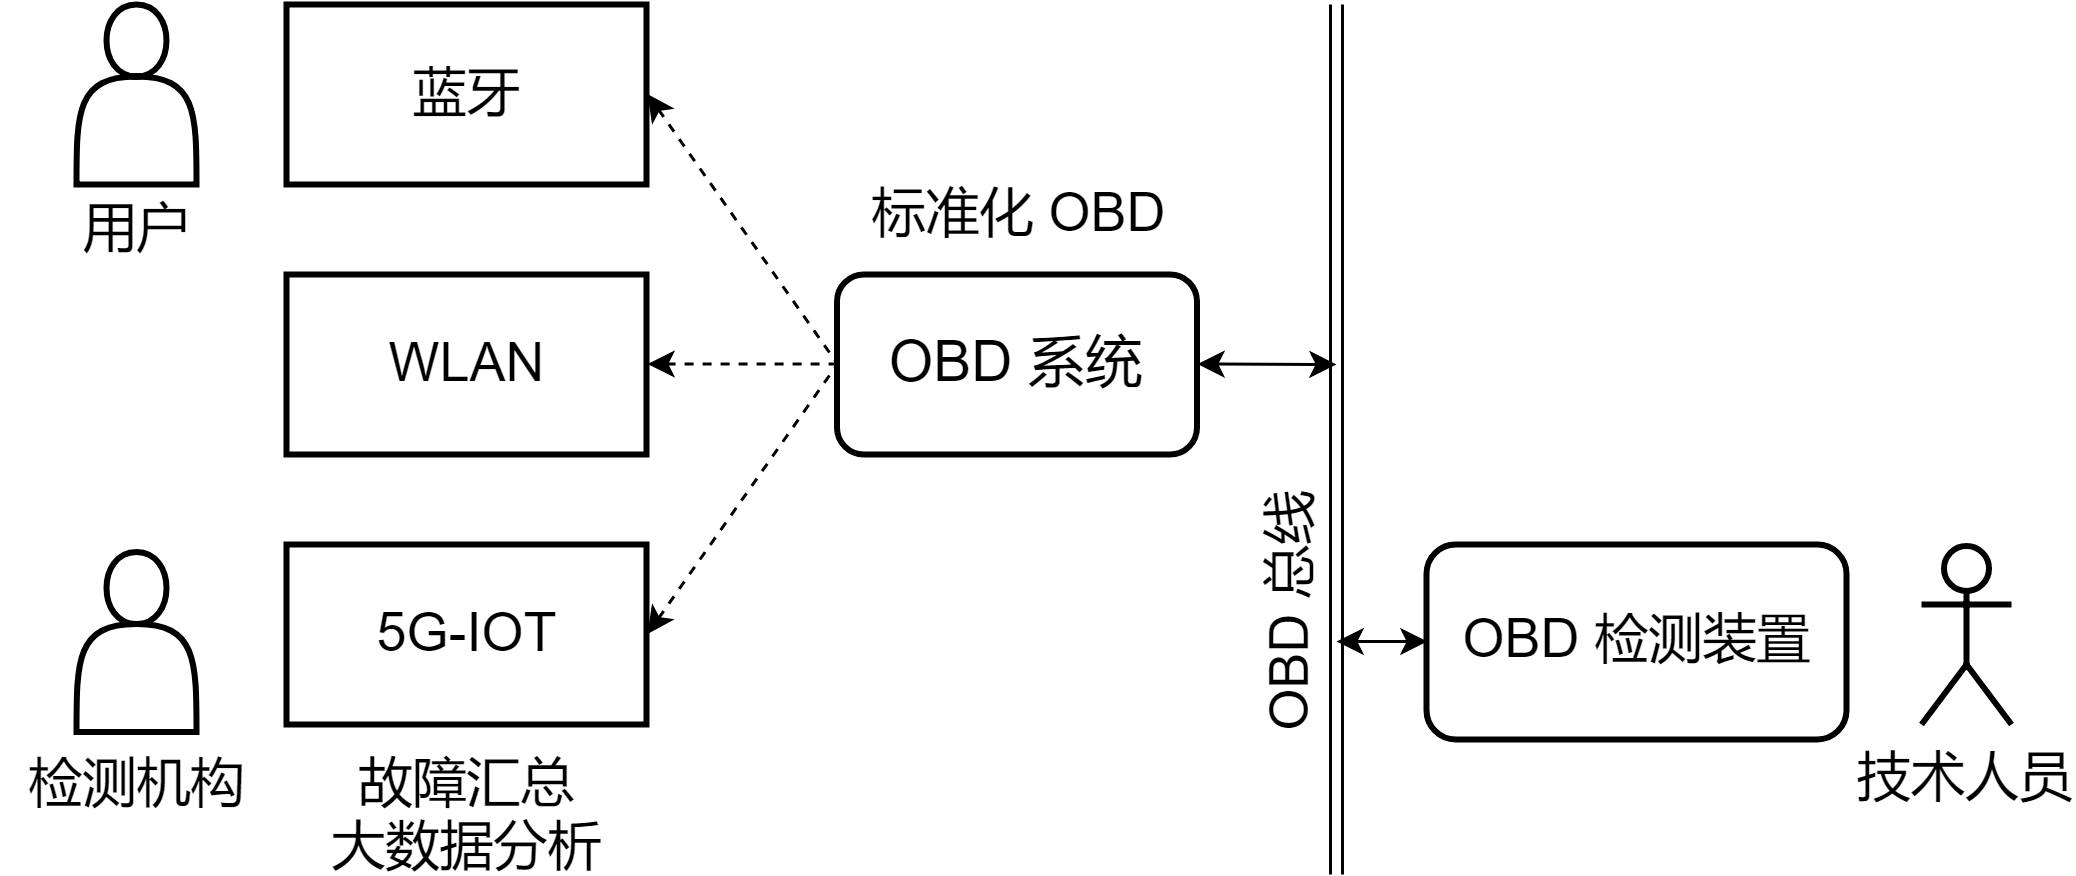
\includegraphics[width=0.7\textwidth]{figures/OBD_future.png}
	\caption{OBD 系统在未来的发展}\label{fig:OBD_future}
\end{figure}

由于电动车技术发展时间较短,故相对于已经在燃油车上使用多年的 OBD 系统来说,电动车的 OBD 系统目前还不太成熟,相关的 ISO 以及 SAE 标准较少。目前已经实施的 OBD 标准,是针对燃油车的排放系统所设置的,对于新的能源系统尚未作出故障的诊断规定。而对于电动车来说,与电动车排放相关的部件即为电池系统和电机系统,所以在传统燃油车上被用作诊断排放相关的 OBD 系统,在目前的电动车上同样应该普及,被用作电池系统和电动机系统的诊断 \cite{Yang2013Research}。

\section{电池箱的 OBD 系统}

电池箱的 OBD 系统是和电池箱的 BMS(Battery Management System 电池管理系统)相协同的。在电池箱内,应该诊断的项目有很多,例如电池箱的箱内温度、压力,开路电压范围,电池的内阻大小,电池的 SOC 范围,电流的大小等等,在诊断之前,OBD 系统需要借助传感器获取这些数据,而 BMS 系统可以通过数据总线提供这些数据,故两个部件必须相互连接;而对于集成 OBD 系统来说,可以在 BMS 系统中设计相应的功能,配合外围的硬件即可实现集成式 OBD 功能。

在目前,电池箱的诊断过程仅仅使用了厂家自行定义的 UDS(Unified Diagnostic Services 统一诊断服务)服务,不同品牌的汽车采用不同的服务码,导致了诊断时不同厂家的车辆产生故障码混乱,而电池箱系统类似于传统油车的发动机,为车辆提供动力,电池箱的故障会引起车辆的能量损耗,故在最新的标准中,为了统一电动汽车诊断流程的规范化,电池箱也被纳入了 OBD 系统的管理范围,在最新的《轻型汽车污染物排放限值及测量方法(中国第六阶段)》(GB 18352.6-2016) \cite{ 轻型汽车污染物排放限值及测量方法(中国第六阶段)} 中的 J.4.14.2.3 部分明确规定了在混合动力汽车中,REESS(电量储存系统)被作为故障检测项目之一,被纳入 OBD 系统必须监测的内容。并且 J.4.14.3 中详细规定了对于电池系统的检测的条件和要求。

综上,可以看到,与其他的诊断协议相比,OBD 诊断系统在协议的规范性、功能性上具有很多优势,在汽车上的应用范围会越来越广,而不仅仅局限于现有的燃油车上。在不久的未来,混合动力汽车将会装配有该系统,而且,可以预测纯电动汽车也会逐渐使用 OBD 系统,OBD 技术将会成为汽车诊断领域的核心技术。

\subsection{物理接口}

在 OBD 相关协议中定义了 OBD 总线使用的物理接口,该接口的形状如图 \ref{fig:OBD_plug} 所示。在 SAE J1962 中规定了该接口的引脚排布,接口的形状为双排 8 Pin 插座,插座的形状有两种类型,被分为 A 型(左)和 B 型(右),不同类型 OBD 接口的引脚的定义相同,并直接接受汽车电池系统供电  \cite{杨沛2017基于OBD接口的低压保护电路}。在此之外,该标准中规定了 OBD 接口必须在转向盘两英尺的范围之内,不得离驾驶员过远。

\begin{figure}
	\centering
	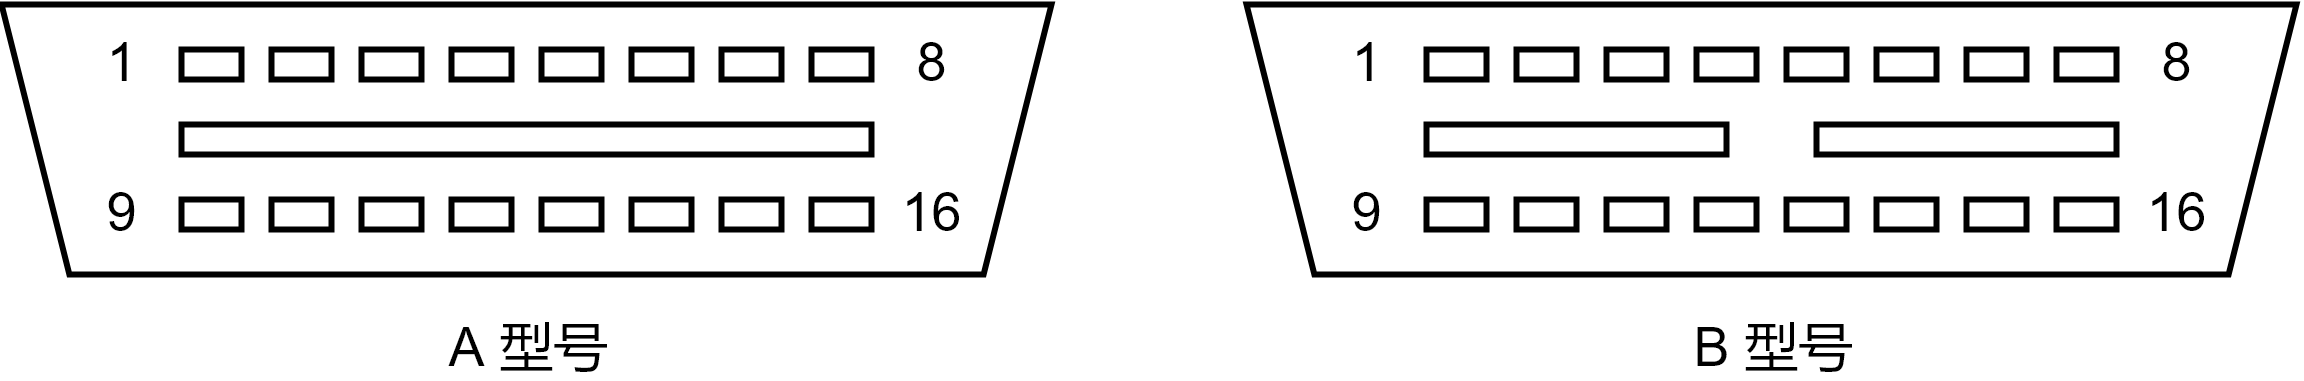
\includegraphics[width=0.7\textwidth]{figures/OBD_plug.png}
	\caption{标准化 OBD 接口}\label{fig:OBD_plug}
\end{figure}

该插座的不同编号的引脚代表了不同的类型,引脚的分布图如表:

\begin{table}
	\centering
	\caption{OBD 引脚定义图} \label{tab:OBD_plug}
	\begin{tabular*}{0.8\textwidth}{@{\extracolsep{\fill}}cc}
		\toprule
		编号			&定义		 \\
		\midrule
		2, 10           & SAE J1850(PWM/VWM)协议总线    \\
		4, 5            & GND(针对所有的协议总线)  \\
        7, 15           & ISO 9141-2/14230-4(KWP2000)协议总线 \\
        6, 14           & ISO 15765-4 (CAN) 协议总线 \\
        16              & 12V Vcc      \\
        其他            & 保留         \\
		\bottomrule
	\end{tabular*}
\end{table}

\subsection{OBD 通信协议电气标准}
在 OBD 系统中,并没有指定特定某一种的协议物理以及链路层的类型,在 OBD 的协议中,可以使用的底层物理和链路层的协议目前可以选择有 3 种,分别为 ISO 9141,也就是目前在旧式汽车上使用的 KWP2000 总线,俗称为 K 线;SAE J1850 中规定的 PWM 和 VPM 协议,又被称之为脉冲宽度调制(Pulse Width Modulation)协议和可变脉冲宽度调制协议(Variable Pulse Width Modulation);ISO 15765-4,基于 CAN 总线的 OBD 协议 \cite{Li2013Design}。

\subsubsection{KWP2000 协议}
在 ISO 9141 中规定了一种被称之为关键字协议 2000 (Keyword Protocol 2000)的标准,它又在 ISO 14230 中被详细规定了物理层和链路层的标准。KWP2000 协议又被称为 K 线通信协议,它是利用一根双向的数据传输线(K-line)。在 K 线(K-line)上,数据以半双工的模式进行通信,其网络结构如图 \ref{fig:OBD_K-line} 所示,在 K 线通信中,可以选择性的增加一根 L 线(L-line),L 线起到唤醒作用。KWP 2000 传输中,将低电平,也就是总线电压小于 $ 20\% Vbus$ 视作逻辑 0;将高电平,也即是总线电压大于 $ 80\% Vbus$ 视作逻辑 1。KWP2000 协议的数据传输速度较慢,其波特率范围为 1.2~10.4 kbps,一次传输可以传输最多 255 字节。由于速度过慢,在 2008 年后,该类型总线不再使用在 OBD 系统上。

\begin{figure}
	\centering
	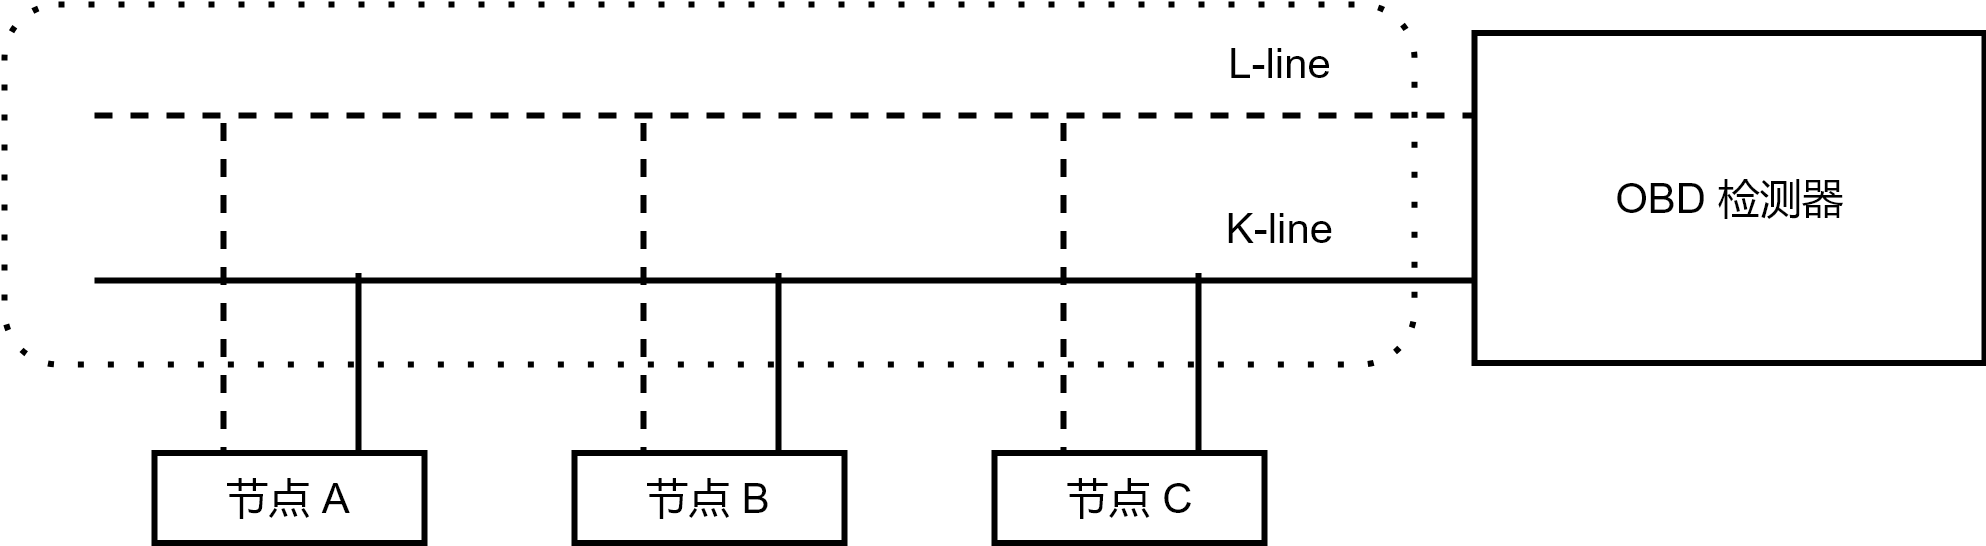
\includegraphics[width=0.7\textwidth]{figures/K-line.png}
	\caption{KWP2000 总线示意图}\label{fig:OBD_K-line}
\end{figure}

\subsubsection{PWM 和 VPM 协议}
PWM 和 VPM 协议是一种应用于 OBD 诊断服务中的总线协议,其标准在 SAE J1850 中被规定,其中使用较多的是基于 PWM 的 OBD 协议。该协议基于脉冲宽度调制原理,利用信号线上每个周期不同的占空比来判断逻辑值。由于 PWM 和 VPM 也是采用单线半双工通信的模式进行通信,通信时速度较慢,PWM 传输速率被固定设定为 41.6 kbps,VPM 传输速率被设定为 10.4 kbps。由于该总线的速度同样较慢,在目前最新生产的车型上,该类型总线已经被淘汰。

\subsubsection{CAN 协议}
CAN 协议作为以上两种协议的替代者,拥有高速,高可靠性的特点。CAN 总线的结构如图 \ref{fig:CAN} 所示,CAN 总线的末端有两个终端电阻,在 ISO 11898-2 中规定了在 高速 CAN 总线上终端电阻的阻值为 120 欧姆。CAN 总线为两线制总线,两根信号线分别被称为 CAN\_High,CAN\_Low。在 CAN 总线上,逻辑值电平有两种,一种被称之为隐性电平,另一种被称为显性电平。隐性电平时,两根线中所有的节点均不驱动信号线,信号线间因为存在终端电阻,故不存在电势差,但是总线的电压值在 2.5V 附近,此时节点检测到无信号,便会认定总线处于空闲状态,或者在传输的过程中,认定总线上的逻辑值为 1;显性电平时,总线上某一节点或多节点将 CAN\_High 信号线驱动向 5V,而将 CAN\_Low 驱动向 0V,在这种情况下,总线上所有的节点都会检测到总线上处于被占有状态,或者在传输数据时,认定总线上的逻辑值为 0。CAN 总线采用两线半双工传输的优势是,信号的判断依靠两根线的共同状态,在传输信号的时候,两根线可以起到差分信号的作用,若总线上发生了电气故障,两根线总线可以快速发现总线故障,提高了传输数据的可靠性。

\begin{figure}
	\centering
	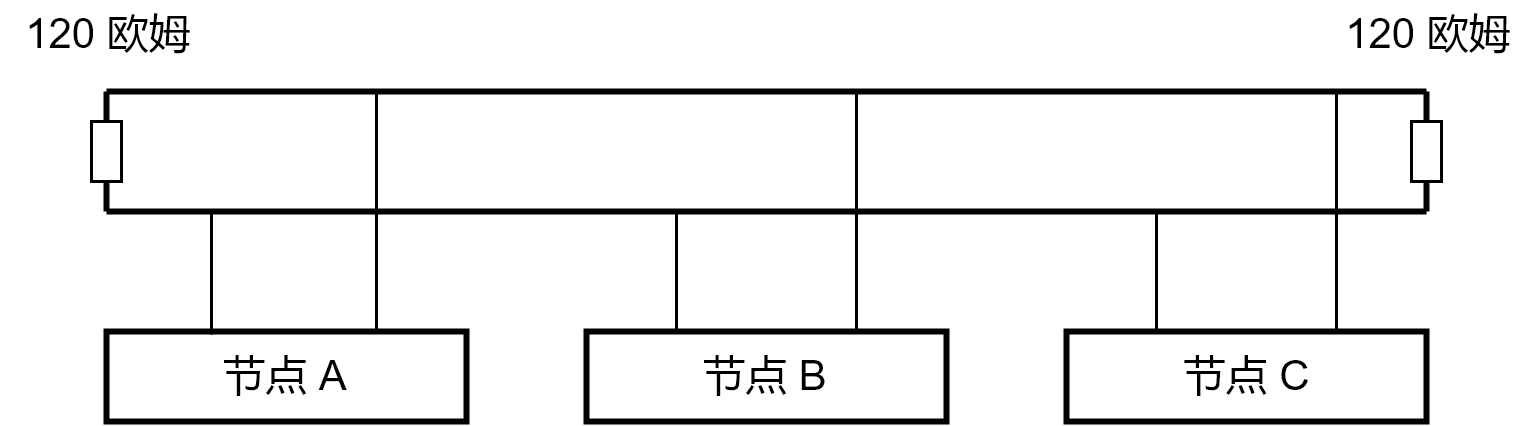
\includegraphics[width=0.7\textwidth]{figures/CAN.png}
	\caption{CAN 总线结构示意图}\label{fig:CAN}
\end{figure}

由于 CAN 总线采用了差分信号机制,与此之外,在数据链路层,CAN 总线提供了一个包含 CRC 校验的信息发送机制,所以 CAN 总线上传输的数据具有相当的可靠性,可以有效抵抗电磁干扰所带来的错误。在发送的时候,传统的总线协议在高速情况下的数据干扰因素在 CAN 总线上被校验机制减弱,故 CAN 总线可以达到更高的传输速率,在 ISO 11898 中规定的高速 CAN 总线信息传输速率最快可以达到 1 mbps。由于 CAN 总线具有优越的性能,故已经被广泛的应用到汽车通信领域,目前几乎所有的车辆都搭载有 CAN 总线。针对此,本文所设计的 OBD 系统是基于 CAN 总线协议的,在物理层和数据链路层使用了标准的 CAN 协议。

\section{OBD 系统设计}
本文所设计的 OBD 系统是符合现行标准的硬件系统,故其通信协议应遵守在 ISO 标准中所定义的 OSI 7 层网络模型结构,如表 \ref{tab:OBD_OSI} 所示。除此之外,在功能上应该具备一套完备的 OBD 系统所应具备的所有功能,包括故障码的储存,MIL 灯的点亮,和响应外置 OBD 诊断仪所提出的 OBD 服务请求功能。

\begin{table}
	\centering
	\caption{OBD OSI 网络结构} \label{tab:OBD_OSI}
	\begin{tabular*}{0.8\textwidth}{@{\extracolsep{\fill}}cc}
		\toprule
		OSI 层			&标准		 \\
		\midrule
		应用层           & ISO 15031-5 / SAE J1979    \\
		展示层           & SAE J2012 DA / SAE J1979 DA \\
        会话层           & ISO 14229-2 \\
        传输层 / 网络层           & ISO 15765-2 \\
        链路层 / 物理层           & ISO 11898      \\
		\bottomrule
	\end{tabular*}
\end{table}

\subsection{硬件配置}
为了满足 OBD 系统的需求,首先需要选择合适的微处理器芯片,同时选择外围的电路需要哪些电子元件。为了实现 OBD 系统中最关键的故障码存储的功能,必须在外围使用一个额外的 NVRAM(非易失性随机访问存储器)来进行故障码的存储,OBD 标准中并未指出应该使用哪一种特定类型的存储器,而为了达成非易失性存储,可以选择的存储器方案有:单独供电的 SRAM 存储区或 DRAM 存储器,EEPROM,或者是使用 Flash 闪存进行存储 \cite{Matas1997Memory}。

\begin{itemize}
	\item 使用单独供电的 SRAM 或 DRAM 存储器,在硬件设计中,应当将微控制器的供电线路和存储器的供电线路分割,使用纽扣电池或者干电池单独对于存储器供电,该方案的优点是,使用该方案的两种 RAM 存储器在存储速度上优于另外两种,数据读写速度在 10 纳秒到 100 纳秒之间。除此优点之外,该方案的存储器读写寿命极长,读取和写入的时候不存在物理损耗现象,故适用于频繁高速大容量读写的应用场所。缺点是该方案的供电线路设计较为复杂,数据的保存需要供电系统进行间隔刷新供电,而且该类型存储器元件价格较高,会提高设计的成本。
	\item 使用 EEPROM 存储器进行数据的存储,EEPROM 又被称作带电可擦可编程只读存储器。该方案的优点为,存储器在断电之后可以保存系统内的数据,并不需要单独的供电,而且成本较低,寿命方面较长,可以达到百万次的写入擦除次数,缺点是容量较小,在市面上可以使用的最大的 EEPROM 容量在 2 MBits 左右,而且读写速度很慢,由于写入时需要一次性写入整个扇区,所以平均的写入时间在数毫秒左右,在高速度的读写应用条件下并不能达到使用要求。
	\item 使用 Flash 存储器,Flash 存储器又被称作闪存,是一种类似于 EEPROM 的非易失性储存器件。Flash 具备 EEPROM 所具备的所有优点,并且与 EEPROM 相比,Flash 储存的单位容量的数据成本更低,写入的速度更快,每次写入一页数据仅仅只有几十微秒,而且 Flash 储存器的价格相当低廉,被广泛的使用于需要储存的各个领域,包括 U 盘,固态硬盘都采用了 Flash 存储器作为存储的介质。但 Flash 存储器的缺点是 Flash 的擦除次数有限,目前常见的 Flash 存储器的擦除次数都在十万次以下。
\end{itemize}

最终本文选择使用 Flash 存储器作为 OBD 系统中的储存器件,因为在 OBD 使用的过程中,数据量较小,但是由于 OBD 系统需要监视实时的数据,数据周期一般只有几十毫秒或者几百毫秒,需要快速的写入和读取,故 EEPROM 并不符合 OBD 的使用需求,而若使用 SRAM 或 DRAM 则会大大增加成本,且需要设计外围的供电电路,使用电池供电,增加了供电所需的成本,而 Flash 价格低廉,而且容量较大,速度也符合 OBD 的应用场景。

\subsection{电路原理图}
电路原理图的完整设计图纸,见附录 A 图 \ref{fig:sheet}。

为了满足调试的需求,在外围使用了来自 FTDI 公司生产的 FT232H 型号芯片,该型号芯片可以通过 USB 接口连接计算机,并且可以同时通过引脚直接访问存储器件,在脱机状态下可以读取 OBD 系统中存储的数据,方便了调试的过程。

\subsubsection{供电电路}
供电电路的设计主要是针对电路板上的各芯片的供电部分进行设计,该电路板的供电方式是使用板载的 USB 接口进行供电,由于 USB 接口的热插拔特性,在插入和拔出的瞬间在线路上会产生较大电流,也会由于静电作用在外壳和电路间产生巨大电压,故在 USB 接口中将数据线 DM DP 用两个 PGB10106603 TVS 瞬态抑制管接地,并且在数据线上使用 0 欧电阻 $R_2$ 和 $R_4$ 作为电路的安全防护作用。USB 接口的 $V_{BUS}$ 引脚为供电电源,其电平为 $5V$,为了抑制该电源线上的高频噪声,在这里使用了规格为 $600R \quad 0.5A$ 的磁珠 $FB_1$,供电电路的设计如图 \ref{fig:USB-SCH} 所示。

\begin{figure}
	\centering
	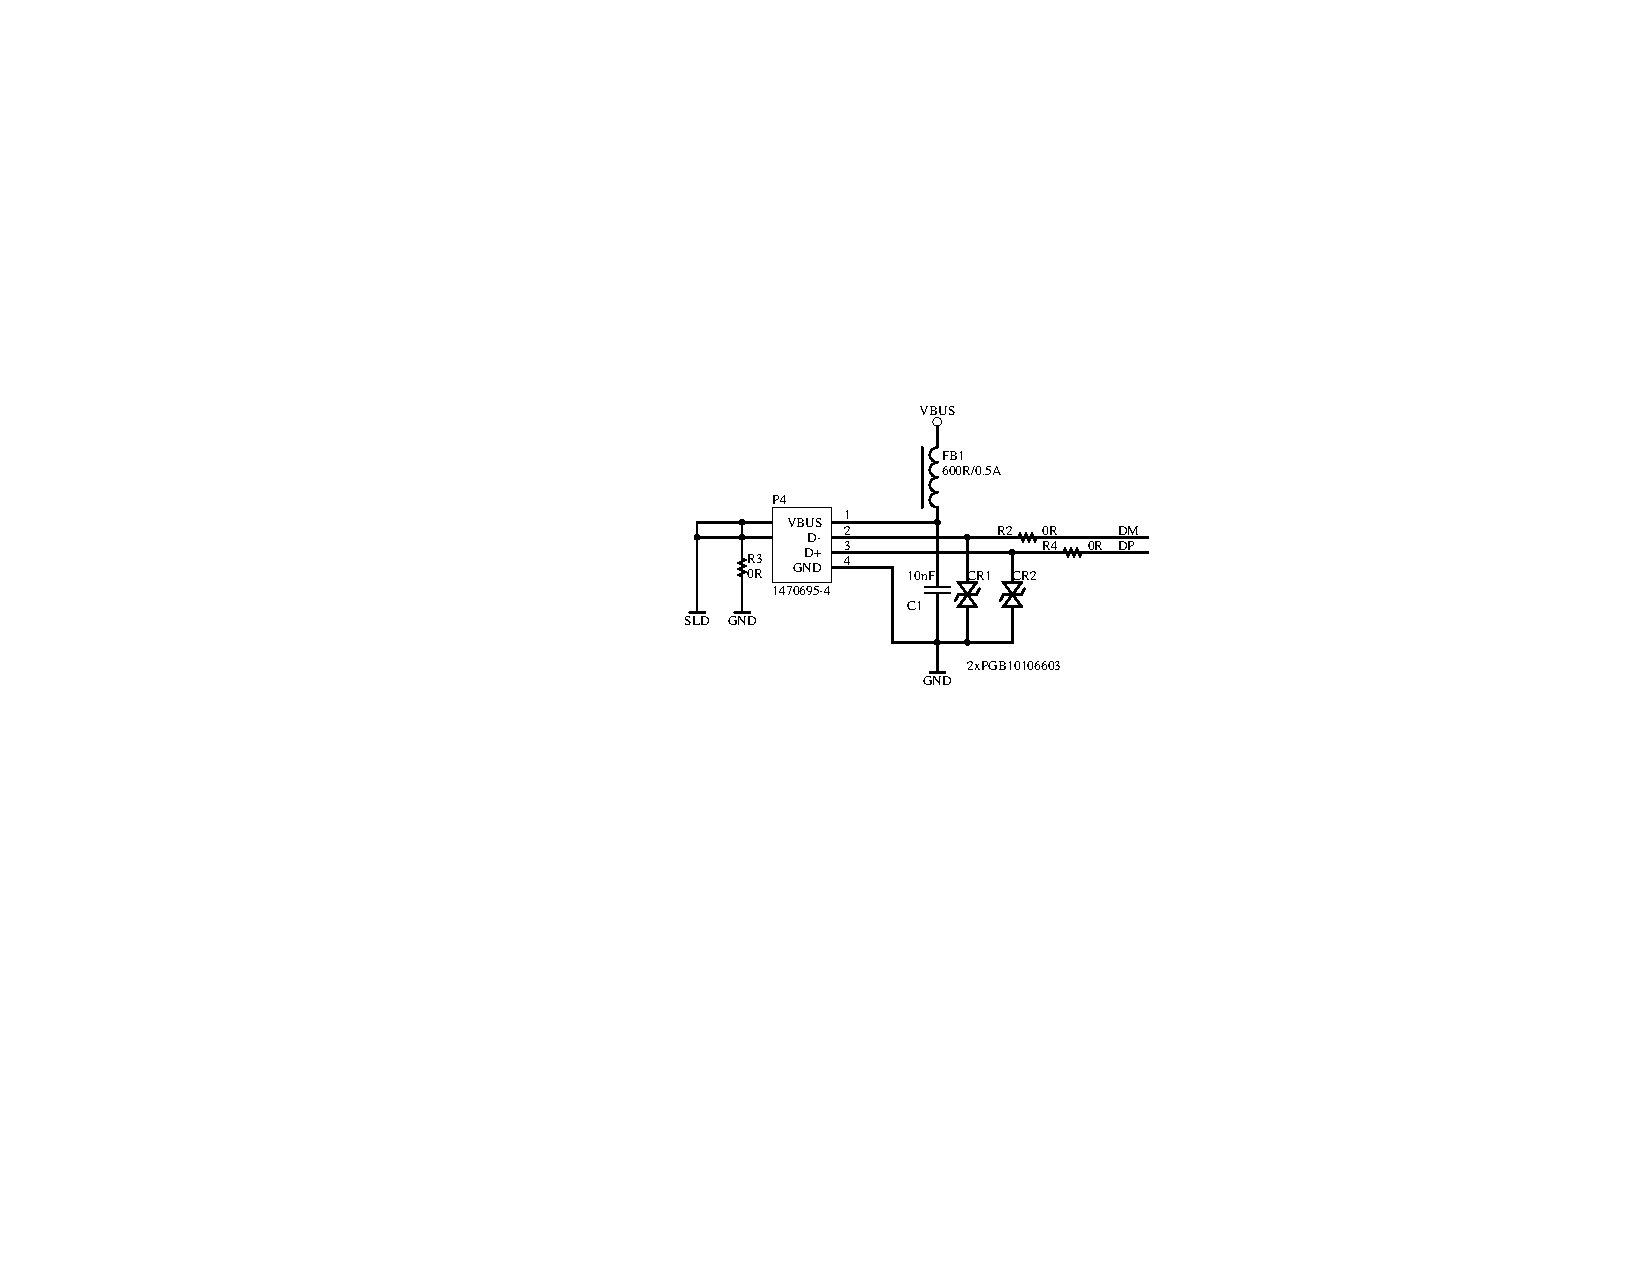
\includegraphics[width=0.5\textwidth]{figures/USB-SCH.pdf}
	\caption{OBD 系统电路供电原理图}\label{fig:USB-SCH}
\end{figure}

在芯片与外围的元器件的滤波电容的设计如图 \ref{fig:filtering-SCH} 所示,其中芯片的 $5V$ 供电电压被内部的 LDO 降压器降压为 $3.3V$ 和 $1.8V$ 供电给芯片自身,故在滤波设计中需要将三种电压分别设置电容滤波网络。

\begin{figure}
	\centering
	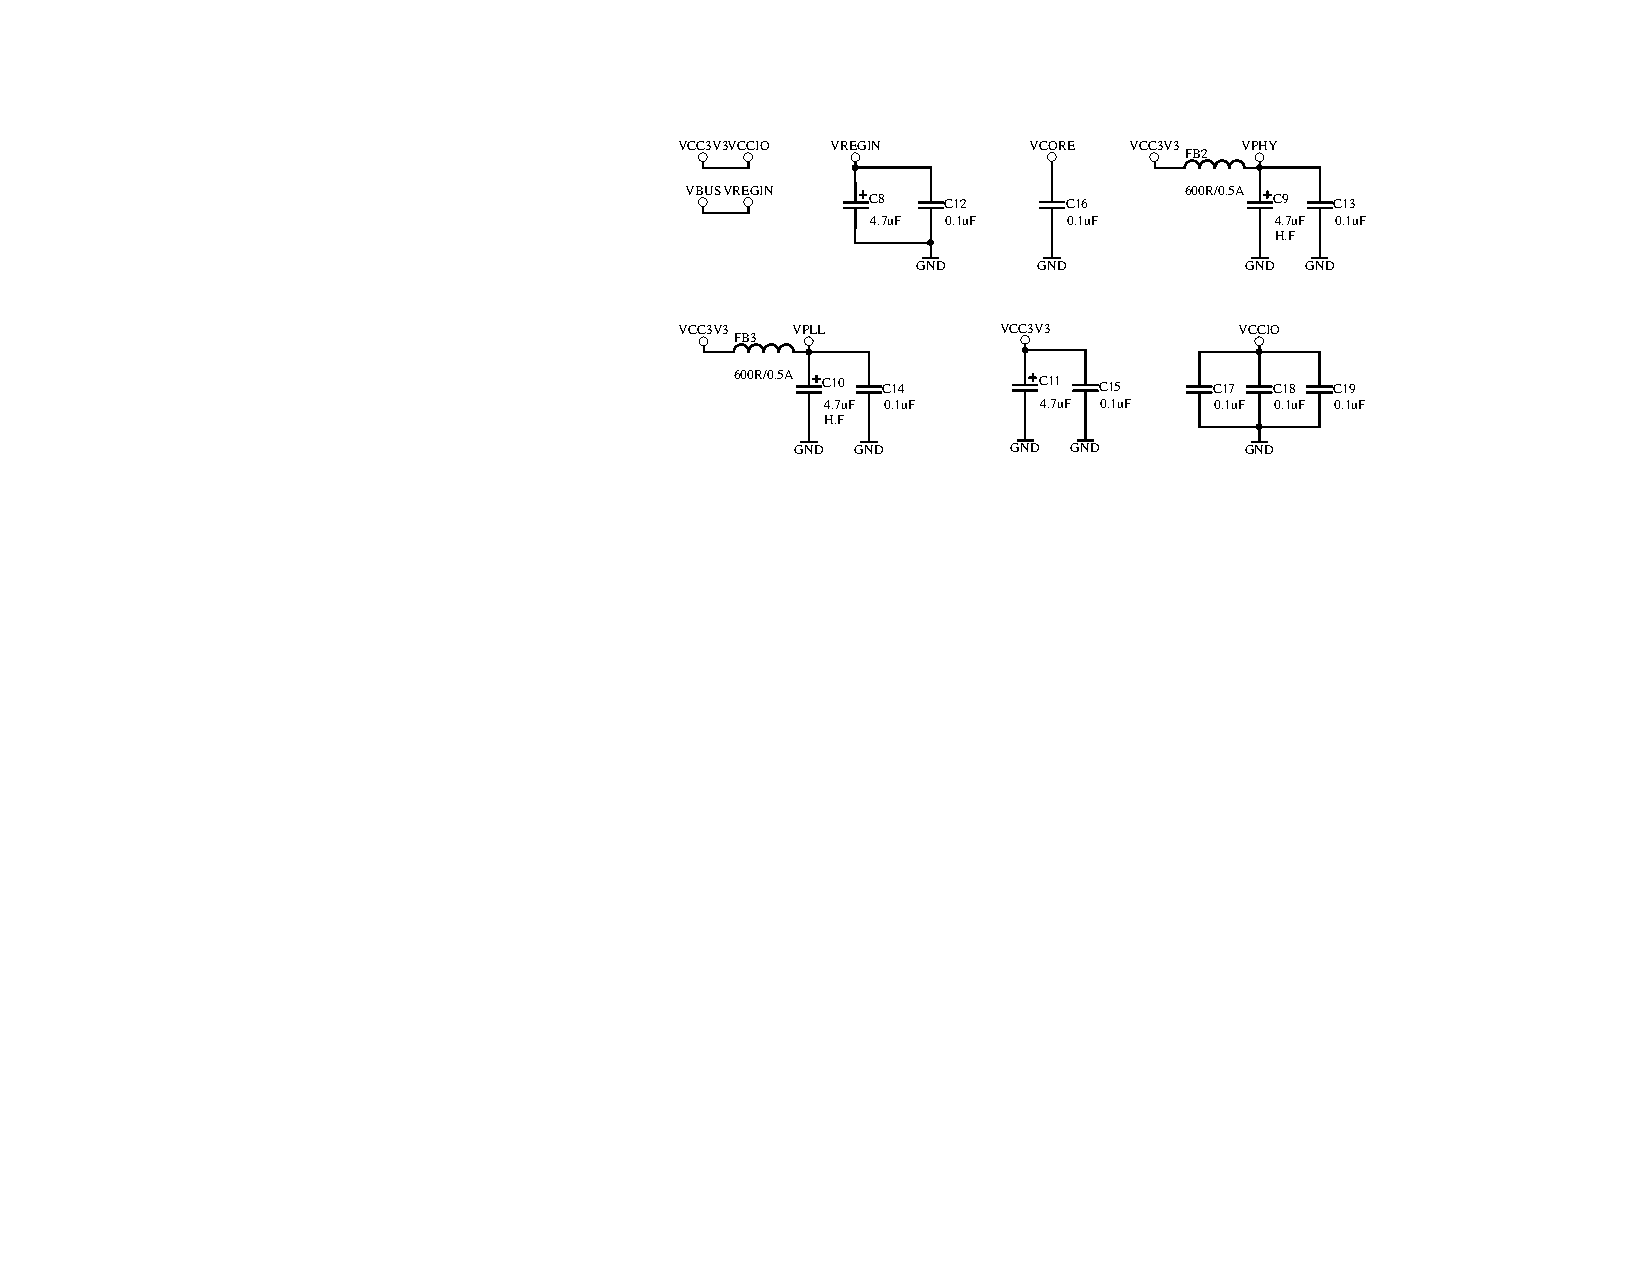
\includegraphics[width=0.5\textwidth]{figures/filtering-SCH.pdf}
	\caption{OBD 系统滤波网络原理图}\label{fig:filtering-SCH}
\end{figure}

\subsubsection{晶振电路}

在电路中晶振使用了 12MHz 的无源晶振,匹配的电容为 $20pF$,电路的设计如图 \ref{fig:XCSIO-SCH}。

\begin{figure}
	\centering
	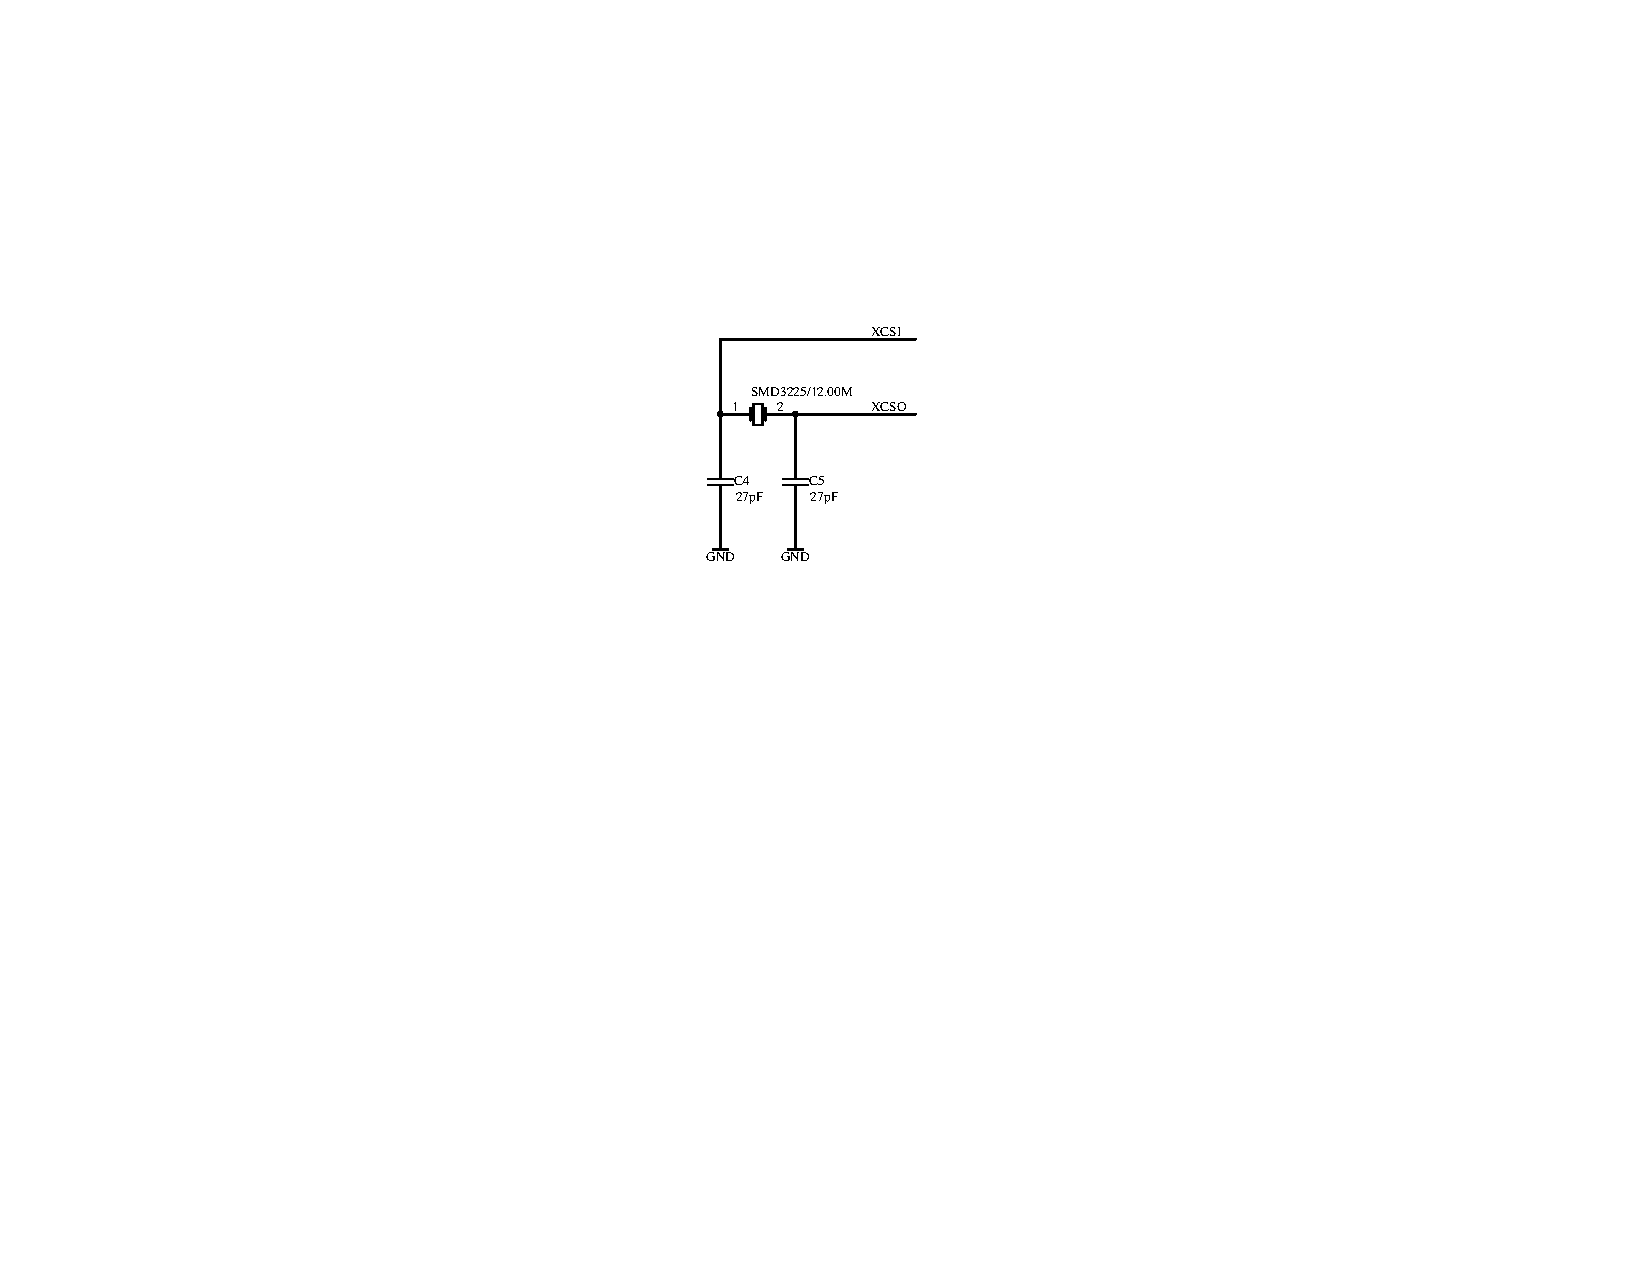
\includegraphics[width=0.5\textwidth]{figures/XCSIO-SCH.pdf}
	\caption{OBD 系统晶振电路原理图}\label{fig:XCSIO-SCH}
\end{figure}

\subsubsection{储存电路}
储存的元器件有两种,一种是被用于存放电路板设置内容的 EEPROM 存储器,另外一种是存放 OBD 故障信息的 Flash 储存器,储存器的电路如图 \ref{fig:EEPROM-SCH} 所示。

\begin{figure}
	\centering
	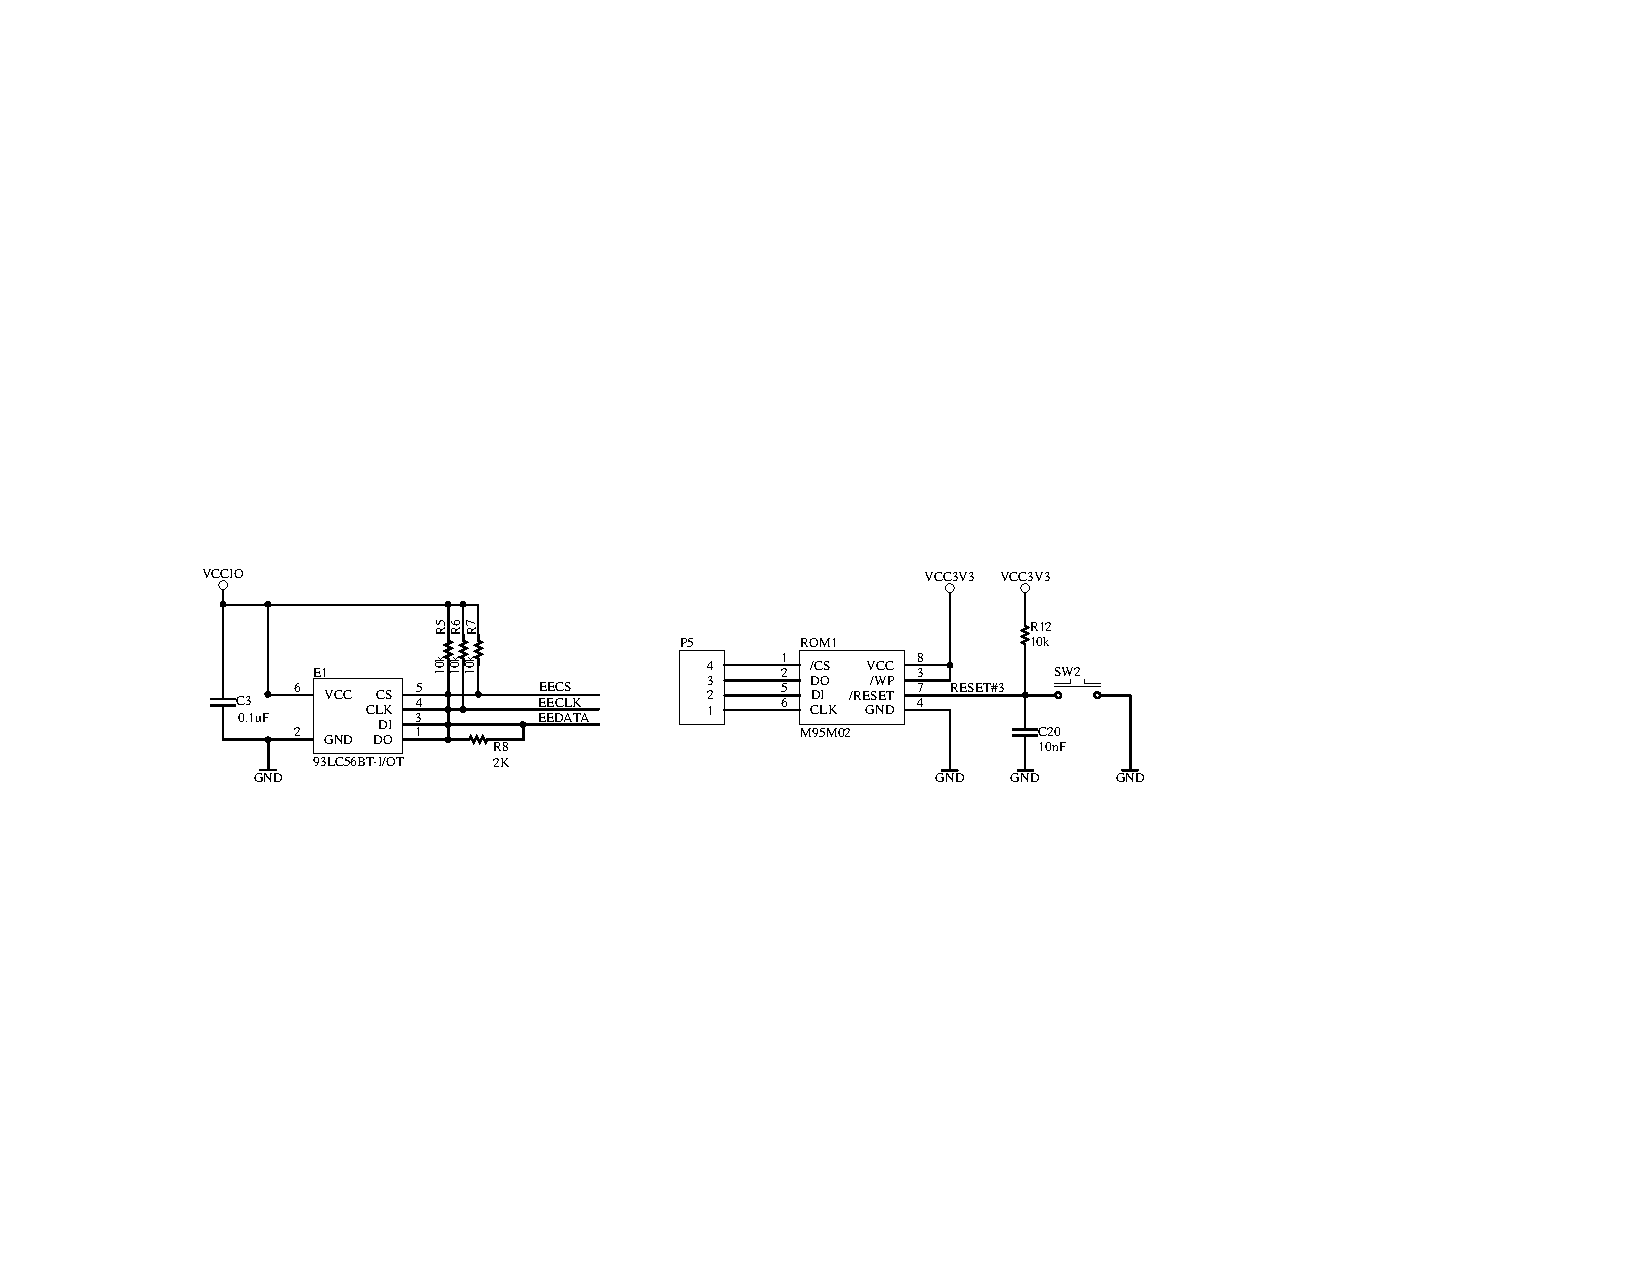
\includegraphics[width=0.35\textwidth]{figures/EEPROM-SCH.pdf}
	\caption{OBD 系统储存原理图}\label{fig:EEPROM-SCH}
\end{figure}

\subsubsection{PCB 电路图}
该 OBD 系统的 PCB 电路图的设计如附录 B 图 \ref{fig:PCB} 所示。该 PCB 电路板已经加工完成,完成了焊接以及调试的过程。

\subsection{OBD 协议栈的开发}
在硬件方面实现了相关功能的元器件的连接之后,在软件层面本文将对于 OBD 协议栈中的设计流程进行简略的介绍。由表 \ref{tab:OBD_OSI} 可以看到首先在在设计 OBD 的软件设计前,需要首先了解 OBD 的网络结构与消息机制。OBD 的网络结构可以分为三个主要的部分,物理层与链路层、网络层与传输层、展示层与应用层,层与层之间的消息传递使用到了 PDU(Protocol Data Unit)协议数据单元为消息的载体。在消息机制方面应该采用消息队列机制,在网络层每部分面设计缓冲数据块,这样系统在高负荷状态下同样可以利用缓冲保证系统稳定性,确保所有的 OBD 服务均能够得到处理,同样提高了系统效率。

\subsubsection{OBD 物理层与链路层}
在 OBD 协议栈中物理层和链路层属于与硬件相关的协议底层 \cite{Zheng2008A},该层协议的实现基于硬件,在 CAN 总线上有 CAN 控制器和 CAN 收发器,其中 CAN 控制器负责数据链路层协议,CAN 收发器负责物理层协议,在市面上常用的单片机中一般集成了 CAN 控制器,可以通过对于单片机中的寄存器的数据控制,通过内置的移位寄存器,达到 CAN 总线的数据发送和接收。

\subsection{OBD 网络层与传输层}
OBD 网络层与传输层主要负责的任务是有关数据传输过程中的以下多个内容:

\begin{itemize}
	\item 数据的多帧分割与重组。
	\item 多帧发送的顺序与流程控制。
	\item 网络参数的设置。
\end{itemize}

众所周知,标注的 CAN2.0A 标准中规定了 CAN 数据帧的数据域长度为 0$\sim$8 个字节,若想要一次性传输多字节,则必须将数据分多帧传输。在 OBD 的网络层与传输层协议中,实现了最长的 4095 个字节的传输。数据在网络层之上的协议层则被抽象成为数据包的格式,不需要考虑数据的传输问题。

多帧传输的过程中,传输的过程较长,在总线上将会进行接收方和发送方的沟通,每隔若干个发送 CAN 帧之后,发送方将会等待接收方发送一个状态指示帧决定接下来的发送数据长度。

网络参数主要是在 OBD 协议网络上的地址参数,如何定义 OBD 节点的地址;OBD 网络的时间参数,发送方应该在一定的时间内响应 OBD 服务以及发起数据传输,而接收方应该设置超时参数,一旦发送方在超时时间内未作出有效的响应,则接收方应该重新发起 OBD 请求。

\subsection{OBD 展示层与应用层}
 OBD 展示层和应用层是面向于用户的内容,该层的开发是 OBD 系统的关键,它决定了 OBD 系统提供给用户的数据,如果将 OBD 系统抽象为网络上的服务器,则用户为客户端,当客户端发起了车辆的诊断请求之后,OBD 系统应该对于该请求作出回应,而应答的内容收到展示层和应用层的标准规定。

OBD 展示层内容主要是车辆故障码的定义以及车辆的诊断过程中如何认定故障的流程,该层的内容需要参考现有的标准包括 SAE J2012 和 ISO 15031-6。OBD 协议应用层的标准包括 SAE J1979 和 ISO 15031-5。在实现的过程中应该遵守标准,这样才能实现报文的通用,不遵守标准会导致系统失去通用性,失去了 OBD 系统的意义。